% Options for packages loaded elsewhere
% Options for packages loaded elsewhere
\PassOptionsToPackage{unicode}{hyperref}
\PassOptionsToPackage{hyphens}{url}
\PassOptionsToPackage{dvipsnames,svgnames,x11names}{xcolor}
%
\documentclass[
  spanish,
  letterpaper,
  DIV=11,
  numbers=noendperiod]{scrartcl}
\usepackage{xcolor}
\usepackage[margin=2cm]{geometry}
\usepackage{amsmath,amssymb}
\setcounter{secnumdepth}{5}
\usepackage{iftex}
\ifPDFTeX
  \usepackage[T1]{fontenc}
  \usepackage[utf8]{inputenc}
  \usepackage{textcomp} % provide euro and other symbols
\else % if luatex or xetex
  \usepackage{unicode-math} % this also loads fontspec
  \defaultfontfeatures{Scale=MatchLowercase}
  \defaultfontfeatures[\rmfamily]{Ligatures=TeX,Scale=1}
\fi
\usepackage{lmodern}
\ifPDFTeX\else
  % xetex/luatex font selection
\fi
% Use upquote if available, for straight quotes in verbatim environments
\IfFileExists{upquote.sty}{\usepackage{upquote}}{}
\IfFileExists{microtype.sty}{% use microtype if available
  \usepackage[]{microtype}
  \UseMicrotypeSet[protrusion]{basicmath} % disable protrusion for tt fonts
}{}
\makeatletter
\@ifundefined{KOMAClassName}{% if non-KOMA class
  \IfFileExists{parskip.sty}{%
    \usepackage{parskip}
  }{% else
    \setlength{\parindent}{0pt}
    \setlength{\parskip}{6pt plus 2pt minus 1pt}}
}{% if KOMA class
  \KOMAoptions{parskip=half}}
\makeatother
% Make \paragraph and \subparagraph free-standing
\makeatletter
\ifx\paragraph\undefined\else
  \let\oldparagraph\paragraph
  \renewcommand{\paragraph}{
    \@ifstar
      \xxxParagraphStar
      \xxxParagraphNoStar
  }
  \newcommand{\xxxParagraphStar}[1]{\oldparagraph*{#1}\mbox{}}
  \newcommand{\xxxParagraphNoStar}[1]{\oldparagraph{#1}\mbox{}}
\fi
\ifx\subparagraph\undefined\else
  \let\oldsubparagraph\subparagraph
  \renewcommand{\subparagraph}{
    \@ifstar
      \xxxSubParagraphStar
      \xxxSubParagraphNoStar
  }
  \newcommand{\xxxSubParagraphStar}[1]{\oldsubparagraph*{#1}\mbox{}}
  \newcommand{\xxxSubParagraphNoStar}[1]{\oldsubparagraph{#1}\mbox{}}
\fi
\makeatother

\usepackage{color}
\usepackage{fancyvrb}
\newcommand{\VerbBar}{|}
\newcommand{\VERB}{\Verb[commandchars=\\\{\}]}
\DefineVerbatimEnvironment{Highlighting}{Verbatim}{commandchars=\\\{\}}
% Add ',fontsize=\small' for more characters per line
\usepackage{framed}
\definecolor{shadecolor}{RGB}{241,243,245}
\newenvironment{Shaded}{\begin{snugshade}}{\end{snugshade}}
\newcommand{\AlertTok}[1]{\textcolor[rgb]{0.68,0.00,0.00}{#1}}
\newcommand{\AnnotationTok}[1]{\textcolor[rgb]{0.37,0.37,0.37}{#1}}
\newcommand{\AttributeTok}[1]{\textcolor[rgb]{0.40,0.45,0.13}{#1}}
\newcommand{\BaseNTok}[1]{\textcolor[rgb]{0.68,0.00,0.00}{#1}}
\newcommand{\BuiltInTok}[1]{\textcolor[rgb]{0.00,0.23,0.31}{#1}}
\newcommand{\CharTok}[1]{\textcolor[rgb]{0.13,0.47,0.30}{#1}}
\newcommand{\CommentTok}[1]{\textcolor[rgb]{0.37,0.37,0.37}{#1}}
\newcommand{\CommentVarTok}[1]{\textcolor[rgb]{0.37,0.37,0.37}{\textit{#1}}}
\newcommand{\ConstantTok}[1]{\textcolor[rgb]{0.56,0.35,0.01}{#1}}
\newcommand{\ControlFlowTok}[1]{\textcolor[rgb]{0.00,0.23,0.31}{\textbf{#1}}}
\newcommand{\DataTypeTok}[1]{\textcolor[rgb]{0.68,0.00,0.00}{#1}}
\newcommand{\DecValTok}[1]{\textcolor[rgb]{0.68,0.00,0.00}{#1}}
\newcommand{\DocumentationTok}[1]{\textcolor[rgb]{0.37,0.37,0.37}{\textit{#1}}}
\newcommand{\ErrorTok}[1]{\textcolor[rgb]{0.68,0.00,0.00}{#1}}
\newcommand{\ExtensionTok}[1]{\textcolor[rgb]{0.00,0.23,0.31}{#1}}
\newcommand{\FloatTok}[1]{\textcolor[rgb]{0.68,0.00,0.00}{#1}}
\newcommand{\FunctionTok}[1]{\textcolor[rgb]{0.28,0.35,0.67}{#1}}
\newcommand{\ImportTok}[1]{\textcolor[rgb]{0.00,0.46,0.62}{#1}}
\newcommand{\InformationTok}[1]{\textcolor[rgb]{0.37,0.37,0.37}{#1}}
\newcommand{\KeywordTok}[1]{\textcolor[rgb]{0.00,0.23,0.31}{\textbf{#1}}}
\newcommand{\NormalTok}[1]{\textcolor[rgb]{0.00,0.23,0.31}{#1}}
\newcommand{\OperatorTok}[1]{\textcolor[rgb]{0.37,0.37,0.37}{#1}}
\newcommand{\OtherTok}[1]{\textcolor[rgb]{0.00,0.23,0.31}{#1}}
\newcommand{\PreprocessorTok}[1]{\textcolor[rgb]{0.68,0.00,0.00}{#1}}
\newcommand{\RegionMarkerTok}[1]{\textcolor[rgb]{0.00,0.23,0.31}{#1}}
\newcommand{\SpecialCharTok}[1]{\textcolor[rgb]{0.37,0.37,0.37}{#1}}
\newcommand{\SpecialStringTok}[1]{\textcolor[rgb]{0.13,0.47,0.30}{#1}}
\newcommand{\StringTok}[1]{\textcolor[rgb]{0.13,0.47,0.30}{#1}}
\newcommand{\VariableTok}[1]{\textcolor[rgb]{0.07,0.07,0.07}{#1}}
\newcommand{\VerbatimStringTok}[1]{\textcolor[rgb]{0.13,0.47,0.30}{#1}}
\newcommand{\WarningTok}[1]{\textcolor[rgb]{0.37,0.37,0.37}{\textit{#1}}}

\usepackage{longtable,booktabs,array}
\usepackage{calc} % for calculating minipage widths
% Correct order of tables after \paragraph or \subparagraph
\usepackage{etoolbox}
\makeatletter
\patchcmd\longtable{\par}{\if@noskipsec\mbox{}\fi\par}{}{}
\makeatother
% Allow footnotes in longtable head/foot
\IfFileExists{footnotehyper.sty}{\usepackage{footnotehyper}}{\usepackage{footnote}}
\makesavenoteenv{longtable}
\usepackage{graphicx}
\makeatletter
\newsavebox\pandoc@box
\newcommand*\pandocbounded[1]{% scales image to fit in text height/width
  \sbox\pandoc@box{#1}%
  \Gscale@div\@tempa{\textheight}{\dimexpr\ht\pandoc@box+\dp\pandoc@box\relax}%
  \Gscale@div\@tempb{\linewidth}{\wd\pandoc@box}%
  \ifdim\@tempb\p@<\@tempa\p@\let\@tempa\@tempb\fi% select the smaller of both
  \ifdim\@tempa\p@<\p@\scalebox{\@tempa}{\usebox\pandoc@box}%
  \else\usebox{\pandoc@box}%
  \fi%
}
% Set default figure placement to htbp
\def\fps@figure{htbp}
\makeatother



\ifLuaTeX
\usepackage[bidi=basic]{babel}
\else
\usepackage[bidi=default]{babel}
\fi
% get rid of language-specific shorthands (see #6817):
\let\LanguageShortHands\languageshorthands
\def\languageshorthands#1{}


\setlength{\emergencystretch}{3em} % prevent overfull lines

\providecommand{\tightlist}{%
  \setlength{\itemsep}{0pt}\setlength{\parskip}{0pt}}



 


\KOMAoption{captions}{tableheading}
\makeatletter
\@ifpackageloaded{caption}{}{\usepackage{caption}}
\AtBeginDocument{%
\ifdefined\contentsname
  \renewcommand*\contentsname{Tabla de contenidos}
\else
  \newcommand\contentsname{Tabla de contenidos}
\fi
\ifdefined\listfigurename
  \renewcommand*\listfigurename{Listado de Figuras}
\else
  \newcommand\listfigurename{Listado de Figuras}
\fi
\ifdefined\listtablename
  \renewcommand*\listtablename{Listado de Tablas}
\else
  \newcommand\listtablename{Listado de Tablas}
\fi
\ifdefined\figurename
  \renewcommand*\figurename{Figura}
\else
  \newcommand\figurename{Figura}
\fi
\ifdefined\tablename
  \renewcommand*\tablename{Tabla}
\else
  \newcommand\tablename{Tabla}
\fi
}
\@ifpackageloaded{float}{}{\usepackage{float}}
\floatstyle{ruled}
\@ifundefined{c@chapter}{\newfloat{codelisting}{h}{lop}}{\newfloat{codelisting}{h}{lop}[chapter]}
\floatname{codelisting}{Listado}
\newcommand*\listoflistings{\listof{codelisting}{Listado de Listados}}
\makeatother
\makeatletter
\makeatother
\makeatletter
\@ifpackageloaded{caption}{}{\usepackage{caption}}
\@ifpackageloaded{subcaption}{}{\usepackage{subcaption}}
\makeatother
\usepackage{bookmark}
\IfFileExists{xurl.sty}{\usepackage{xurl}}{} % add URL line breaks if available
\urlstyle{same}
\hypersetup{
  pdftitle={Lección 1: Introducción a los datos},
  pdfauthor={Hans Sigrist},
  pdflang={es},
  colorlinks=true,
  linkcolor={blue},
  filecolor={Maroon},
  citecolor={Blue},
  urlcolor={blue},
  pdfcreator={LaTeX via pandoc}}


\title{Lección 1: Introducción a los datos}
\author{Hans Sigrist}
\date{2026-03-05}
\begin{document}
\maketitle
\begin{abstract}
En esta lección se estudia un experimento clínico sobre el uso de stents
para prevenir accidentes cerebrovasculares. Se introducen las nociones
de variable explicativa y variable respuesta, así como el uso de tablas
de contingencia y proporciones. Mediante el entorno R y el paquete
openintro se desarrollan procedimientos básicos para organizar y resumir
datos. El propósito es iniciar la comprensión del análisis estadístico
en contextos descriptivos e inferenciales.
\end{abstract}

\renewcommand*\contentsname{Tabla de contenidos}
{
\hypersetup{linkcolor=}
\setcounter{tocdepth}{3}
\tableofcontents
}

Built with Quarto v1.8.27 · R v4.5.2 · tidyverse v2.0.0 · LaTeX
v3.141592653-2.6-1.40.27 · openintro v2.5.0

\begin{figure}

\centering{

\pandocbounded{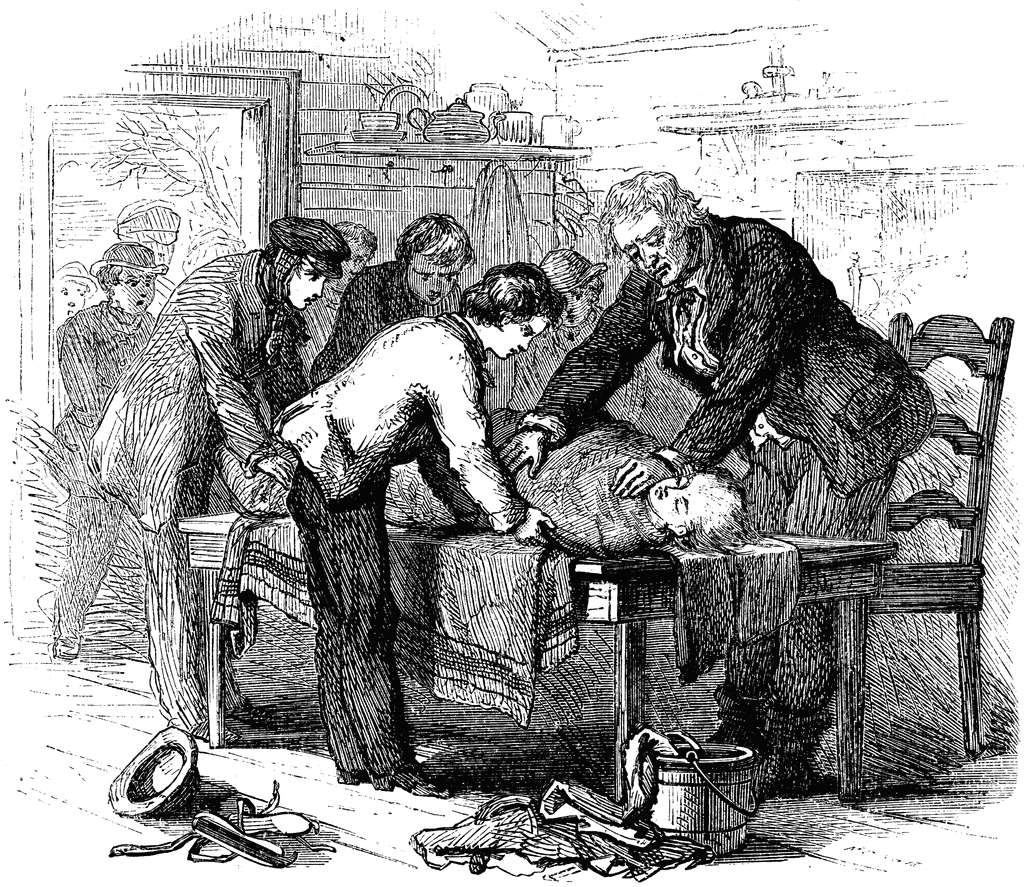
\includegraphics[keepaspectratio]{../imagenes/65138_patient_lg.png}}

}

\caption{\label{fig-railroad-pdf}Ilustración utilizada con fines
educativos. Fuente: USF ClipArt Collection (University of South
Florida).}

\end{figure}%

\section{Google Colaboratory (Colab)}\label{google-colaboratory-colab}

\href{https://colab.google/}{colab} es un servicio alojado de
\href{https://jupyter.org/}{Jupyter Notebook} que no requiere
configuración y ofrece acceso gratuito a recursos informáticos, como GPU
y TPU. Colab es especialmente adecuado para el aprendizaje automático,
la ciencia de datos y la educación.

En esta asignatura, lo utilizaremos para representar, graficar y resumir
datos que no es posible implementar en otras aplicaciones como Excel u
Hojas de Cálculo de Google (al menos sin la fricción propia de éstos).

Pero \textbf{colab} solo es el espacio de trabajo, necesitamos un motor,
un lenguaje que compile nuestros datos. Actualmente, existen dos
principalmente que permiten desarrollar análisis matemático y/o
estadístico: \href{https://www.python.org/}{python} y
\href{https://www.r-project.org/}{R}.

Usualmente, un usuario interesado en ejecutar este tipo de programas
necesita:

\begin{enumerate}
\def\labelenumi{\arabic{enumi}.}
\tightlist
\item
  Un \textbf{editor}
\item
  Un \textbf{kernel}
\item
  Conocer los \textbf{comandos del lenguaje} correspondiente
\end{enumerate}

Con \textbf{colab} contamos con los dos primeros recursos: (1)
\textbf{colab} en sí es un editor y (2) Google ofrece por medio de sus
servicios distintos kernel, entre ellos python y R. Es cosa de
``instalarlos'' (en realidad nada se instala en tu computador solo se
instalan en el servidor) y luego (3) usar los comandos respectivos para
manipular datos -por ejemplo.

\section{Tu cuenta institucional}\label{tu-cuenta-institucional}

Solo necesitas eso, tu cuenta institucional @colegioportaliano.cl:

\begin{enumerate}
\def\labelenumi{\arabic{enumi}.}
\tightlist
\item
  Ingresa en \href{https://colab.google/}{colab}
\item
  Presiona el botón ``New Notebook'', te advertirá que se requiere el
  acceso a Google y presionas el botón Acceder.
\item
  Ingresas tus credenciales, posiblemente te solicite que ingreses un
  segundo nivel de seguridad (mensaje de texto en tu celular, presionar
  ``si'' en un celular, etc.)
\item
  Listo ya estás en \textbf{colab}.
\end{enumerate}

\section{R}\label{r}

\href{https://www.r-project.org}{R} es un entorno de software libre para
computación estadística y gráficos. Se compila y ejecuta en una amplia
variedad de plataformas UNIX, Windows y macOS. Este será nuestro kernel
por defecto. Y por sus características, versatilidad y amplios usos en
ciencias, economía, salud, ingeniería, etc. es alimentado por una gran
comunidad que provee paquetes o librerías de dedicación especial. ¿Qué
significa esto? Bueno, que usuarios alrededor del mundo han facilitado
mucho las cosas para que otros usuarios -como ustedes y yo- podamos
utilizar bases de datos originales y actualizadas que junto con la
potencia del kernel R nos permiten realizar simulaciones que no
podríamos hacer con otros software convencionales (mucha fricción).

Y eso es justamente lo que haremos ahora. Prepárate.

\section{Estudio de caso: uso de stent para prevenir ACV (accidente
cerebrovascular)}\label{estudio-de-caso-uso-de-stent-para-prevenir-acv-accidente-cerebrovascular}

En esta sección, consideraremos un experimento que estudia la eficacia
de los stents (también conocido como \emph{endoprótesis vascular}: una
malla o férula diseñada para abrir arterias, venas u otros conductos
estrechados o bloqueados) en el tratamiento de pacientes con riesgo de
ACV. Los stents son dispositivos que se colocan dentro de los vasos
sanguíneos y que facilitan la recuperación del paciente tras un evento
cardíaco y reducen el riesgo de sufrir otro ACV o incluso la muerte.
Muchos médicos esperaban que se obtuvieran beneficios similares para los
pacientes con riesgo de ACV.

Comenzamos por escribir la \emph{pregunta principal} que los
investigadores esperan responder:

\textbf{¿Reduce el uso de stents el riesgo de un ACV?}

\subsection{El experimento}\label{el-experimento}

Los investigadores que formularon esta pregunta realizaron un
experimento con \(451\) pacientes en riesgo.

Cada paciente voluntario fue asignado aleatoriamente a uno de dos
grupos:

\begin{itemize}
\tightlist
\item
  \textbf{Grupo de tratamiento.} Los pacientes del grupo de tratamiento
  recibieron un stent y tratamiento médico. El tratamiento médico
  incluyó medicamentos, control de los factores de riesgo y ayuda para
  modificar el estilo de vida.
\item
  \textbf{Grupo de control.} Los pacientes del grupo de control
  recibieron el mismo tratamiento médico que el grupo de tratamiento,
  pero no recibieron stents.
\end{itemize}

Los investigadores asignaron aleatoriamente a \(224\) pacientes al grupo
de tratamiento y a \(227\) al grupo de control.

En este estudio, el grupo de control proporciona un punto de referencia
para medir el impacto médico de los stents en el grupo de tratamiento.

Los investigadores estudiaron el efecto de los stents en dos momentos:
\(30\) días después de la inscripción y \(365\) días después de la
inscripción.

\subsection{El resumen}\label{el-resumen}

Los resultados de 5 pacientes se resumen en la tabla
Tabla~\ref{tbl-stent-data}. Los resultados de los pacientes se registran
como ``stroke'' o ``no event'', lo que indica si el paciente sufrió o no
un ACV al final de un período.

\begin{longtable}[]{@{}clcc@{}}
\caption{Tabla de resultados por paciente en el estudio de
stents}\label{tbl-stent-data}\tabularnewline
\toprule\noalign{}
Patient & Group & 0--30 days & 0--365 days \\
\midrule\noalign{}
\endfirsthead
\toprule\noalign{}
Patient & Group & 0--30 days & 0--365 days \\
\midrule\noalign{}
\endhead
\bottomrule\noalign{}
\endlastfoot
1 & treatment & no event & no event \\
2 & treatment & stroke & stroke \\
3 & treatment & no event & no event \\
⋮ & ⋮ & ⋮ & ⋮ \\
450 & control & no event & no event \\
451 & control & no event & no event \\
\end{longtable}

\subsection{Primer problema}\label{primer-problema}

Considerar los datos de cada paciente individualmente sería un proceso
largo y engorroso para responder a la pregunta de investigación
original.

En cambio, realizar un análisis estadístico de datos nos permite
considerar todos los datos a la vez.

Aquí entra R.

Existe una librería llamada ``openintro'' que a su vez es la creadora de
muchas bases de datos, entre ellas stent30 y stent365, para usarlas
debemos primero, instalar la librería:

Presiona Shift+Enter dentro de esta celda (usualmente al final del
texto):

\begin{Shaded}
\begin{Highlighting}[]
\FunctionTok{install.packages}\NormalTok{(}\StringTok{"openintro"}\NormalTok{)}
\end{Highlighting}
\end{Shaded}

Podrás ver cómo colab instala la librería y sus componentes e incluso
algunas otras cosas que necesita para su funcionamiento (dependencias).
Puede durar desde algunos pocos segundos hasta un minuto
aproximadamente. No hagas nada, solo espera que termine.

Ya instalada la librería, debemos invocarla:

\begin{Shaded}
\begin{Highlighting}[]
\FunctionTok{library}\NormalTok{(openintro)}
\end{Highlighting}
\end{Shaded}

\begin{verbatim}
Cargando paquete requerido: airports
\end{verbatim}

\begin{verbatim}
Cargando paquete requerido: cherryblossom
\end{verbatim}

\begin{verbatim}
Cargando paquete requerido: usdata
\end{verbatim}

Listo, librería activa. No se observa nada.

Para inspeccionar qué contiene esta librería usamos el comando
\texttt{data()}:

\begin{Shaded}
\begin{Highlighting}[]
\FunctionTok{data}\NormalTok{(}\AttributeTok{package =} \StringTok{"openintro"}\NormalTok{)}
\end{Highlighting}
\end{Shaded}

Se desplegará un menú vertical a la derecha con todos los conjuntos de
datos del paquete ``openintro'' y su descripción. Si navegas podrás ver
a stent30 y a stent365.

Ahora carguemos nuestras bases de datos de estudio, recuerda que son de
la librería openintro. Usamos \texttt{data()} nuevamente:

\begin{Shaded}
\begin{Highlighting}[]
\FunctionTok{data}\NormalTok{(stent30,stent365)}
\end{Highlighting}
\end{Shaded}

Un comando útil en estos momentos es \texttt{ls()}, éste lista el
contenido cargado:

\begin{Shaded}
\begin{Highlighting}[]
\FunctionTok{ls}\NormalTok{()}
\end{Highlighting}
\end{Shaded}

\begin{verbatim}
[1] "stent30"  "stent365"
\end{verbatim}

Podrás ver la salida:
\texttt{\textquotesingle{}stent30\textquotesingle{}} y
\texttt{\textquotesingle{}stent365\textquotesingle{}}

Ahora queremos saber qué estructura tiene el archivo, pues aún no lo
vemos. Para ello usamos \texttt{str()}:

\begin{Shaded}
\begin{Highlighting}[]
\FunctionTok{print}\NormalTok{(}\FunctionTok{str}\NormalTok{(stent365))}
\end{Highlighting}
\end{Shaded}

\begin{verbatim}
tibble [451 x 2] (S3: tbl_df/tbl/data.frame)
 $ group  : Factor w/ 2 levels "control","treatment": 2 2 2 2 2 2 2 2 2 2 ...
 $ outcome: Factor w/ 2 levels "no event","stroke": 2 2 2 2 2 2 2 2 2 2 ...
NULL
\end{verbatim}

Interpretación: se trata de una tabla de dos factores, cada uno con dos
niveles.

¿Podrías decir cuáles son cada uno?

También podemos usar el comando \texttt{head()} que nos muestra el
encabezado de la tabla:

\begin{Shaded}
\begin{Highlighting}[]
\FunctionTok{head}\NormalTok{(stent365)}
\end{Highlighting}
\end{Shaded}

\begin{verbatim}
# A tibble: 6 x 2
  group     outcome
  <fct>     <fct>  
1 treatment stroke 
2 treatment stroke 
3 treatment stroke 
4 treatment stroke 
5 treatment stroke 
6 treatment stroke 
\end{verbatim}

¿Cómo interpretas lo anterior?

Justo en este momento sería bueno que ejecutaras el siguiente comando
que te permitirá conocer finalmente la base de datos \texttt{stent365}:

\begin{Shaded}
\begin{Highlighting}[]
\FunctionTok{write.csv}\NormalTok{(stent30,  }\StringTok{"stent30.csv"}\NormalTok{,  }\AttributeTok{row.names =} \ConstantTok{FALSE}\NormalTok{)}
\FunctionTok{write.csv}\NormalTok{(stent365, }\StringTok{"stent365.csv"}\NormalTok{, }\AttributeTok{row.names =} \ConstantTok{FALSE}\NormalTok{)}
\FunctionTok{list.files}\NormalTok{(}\AttributeTok{pattern =} \StringTok{"\^{}stent(30|365)}\SpecialCharTok{\textbackslash{}\textbackslash{}}\StringTok{.csv$"}\NormalTok{)}
\end{Highlighting}
\end{Shaded}

\begin{verbatim}
[1] "stent30.csv"  "stent365.csv"
\end{verbatim}

Ahora ve al panel de la izquierda y abre el penúltimo ícono Archivos,
actualiza y verás dos nuevos archivos para descargar. ¿Te diste cuenta?
Es simplemente un archivo \texttt{csv} (comma separated values) de
valores separados por coma, que leídos por esta hoja de cálculo
corresponden simplemente a dos columnas de datos.

Por las características de los datos (estructura, encabezados,
extensión), a veces es imposible usar hojas de cálculo para su lectura.
Eso es justamente lo que estamos haciendo aquí. Como ambas variables son
categóricas, el resumen natural es una tabla de contingencia (doble
entrada).

Para una tabla de contingencia usamos el comando \texttt{table()} de
esta forma:

\begin{Shaded}
\begin{Highlighting}[]
\NormalTok{tab\_stent365 }\OtherTok{\textless{}{-}} \FunctionTok{table}\NormalTok{(stent365}\SpecialCharTok{$}\NormalTok{group, stent365}\SpecialCharTok{$}\NormalTok{outcome)}
\NormalTok{tab\_stent365}
\end{Highlighting}
\end{Shaded}

\begin{verbatim}
           
            no event stroke
  control        199     28
  treatment      179     45
\end{verbatim}

Con la primera linea estamos pidiendo a R que use el comando
\texttt{table()} para agrupar tanto por group como por outcome. Con la
segunda linea, le pedimos que muestre dicha tabla.

Intenta hacer algunos simples cálculos aritméticos y te
sorprenderás\ldots{}

Ahora haremos algo más matemático y desde el punto de vista estadístico
muy importante. Introduciremos la probabilidad, en este contexto: la
proporción de pacientes según el grupo y el nivel.

Para ello usamos el comando \texttt{prop.table()} de esta forma:

\begin{Shaded}
\begin{Highlighting}[]
\FunctionTok{prop.table}\NormalTok{(tab\_stent365, }\AttributeTok{margin =} \DecValTok{1}\NormalTok{)}
\end{Highlighting}
\end{Shaded}

\begin{verbatim}
           
             no event    stroke
  control   0.8766520 0.1233480
  treatment 0.7991071 0.2008929
\end{verbatim}

Esta vez no copiaré el resultado porque ya te has dado cuenta de que son
exactamente las salidas de los comandos que he ido proponiéndote.

A partir de tabla, ¿Qué estás observando? ¿Cómo lo interpretas? ¿Podrías
hacer una conclusión? ¿Podrías responder a la pregunta inicial?

Para ayudar a tus conclusiones, siempre es bueno una perspectiva visual
de la problemática. Para ello usamos el comando \texttt{barplot()} de
esta forma:

\begin{Shaded}
\begin{Highlighting}[]
\FunctionTok{barplot}\NormalTok{(}\FunctionTok{prop.table}\NormalTok{(tab\_stent365, }\DecValTok{1}\NormalTok{),}
        \AttributeTok{beside =} \ConstantTok{FALSE}\NormalTok{,}
        \AttributeTok{legend =} \ConstantTok{TRUE}
\NormalTok{)}
\end{Highlighting}
\end{Shaded}

\pandocbounded{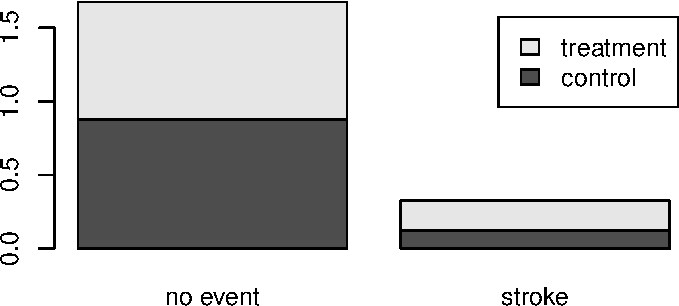
\includegraphics[keepaspectratio]{leccion-1-introduccion-a-los-datos_files/figure-pdf/unnamed-chunk-11-1.pdf}}

¿Te atreves ahora a responder a la pregunta inicial? Escribe tu
respuesta en tu cuaderno y compártela cuando se te solicite.

\section{Cuestionario}\label{cuestionario}

\begin{enumerate}
\def\labelenumi{\arabic{enumi}.}
\item
  Explica con tus palabras cuál era la pregunta de investigación y por
  qué los médicos necesitaban un experimento para responderla, en lugar
  de confiar solo en su intuición.
\item
  Identifica la \textbf{variable explicativa} y la \textbf{variable
  respuesta} del estudio. ¿Por qué la primera se llama ``explicativa'' y
  la segunda ``respuesta''?
\item
  ¿Qué problema resuelve la \textbf{asignación aleatoria} de los
  pacientes a los grupos? ¿Qué podría haber pasado si los médicos
  hubieran decidido qué paciente recibe stent y cuál no?
\item
  Sin un \textbf{grupo de control}, ¿podríamos saber si los stents
  realmente causaron alguna diferencia? Explica por qué.
\item
  Clasifica las variables \texttt{group} y \texttt{outcome} según su
  naturaleza (cuantitativas discretas, continuas, categóricas nominales
  u ordinales). Justifica cada clasificación.
\item
  ¿Por qué estos datos se resumen naturalmente en una \textbf{tabla de
  contingencia} y no, por ejemplo, en un promedio o una mediana?
\item
  Con los datos del estudio (224 tratamiento, 45 ACV; 227 control, 28
  ACV):

  \begin{enumerate}
  \def\labelenumii{\alph{enumii})}
  \tightlist
  \item
    Calcula la proporción de ACV en cada grupo.
  \item
    Calcula la diferencia entre ambas proporciones.
  \item
    A la luz de estos números, ¿dirías que los stents reducen el riesgo
    de ACV? ¿Por qué?
  \end{enumerate}
\item
  La diferencia que calculaste, ¿podría deberse simplemente al azar?
  Explica usando un ejemplo simple, como lanzar una moneda.
\item
  Si el estudio hubiera tenido muchos menos pacientes, ¿confiarías más o
  menos en el resultado? ¿Por qué?
\item
  Los pacientes fueron \textbf{voluntarios}. ¿Podemos estar seguros de
  que estos resultados se aplican a \emph{todos} los pacientes con
  riesgo de ACV? Explica.
\item
  El estudio encontró ``evidencia convincente de daño'' en lugar de
  beneficio. ¿Qué significa esta frase en el contexto de los stents?
\item
  Calcula la \textbf{razón de proporciones} (tratamiento / control). Un
  valor mayor que 1 indica mayor riesgo en el grupo tratamiento. ¿Qué
  obtuviste? Interprétalo.
\item
  Si el stent realmente redujera el riesgo de ACV, ¿qué esperarías ver
  en las proporciones y en la razón que calculaste?
\item
  Menciona dos \textbf{limitaciones} del estudio que podrían afectar la
  confianza en sus conclusiones.
\item
  ¿Qué enseñanza deja este caso sobre la relación entre la
  \textbf{intuición médica} y la \textbf{evidencia estadística}? Escribe
  una reflexión breve.
\end{enumerate}




\end{document}
